\documentclass[xetex,svgnames]{scrartcl}

% packages
\usepackage{xltxtra}
\usepackage{polyglossia}
\usepackage[
    urlcolor=black,
    linkcolor=black,
    citecolor=black,
    filecolor=black,
    pagecolor=black,
    linktocpage=true,
    ]{hyperref}
\usepackage{fontspec}
\usepackage{scrpage2}
\usepackage[left=2cm,right=2cm,top=3cm,bottom=3cm]{geometry}
\usepackage{colortbl,color,xcolor}
\usepackage{alltt}
\usepackage{listings}
\usepackage{multirow}
\usepackage{csquotes}

% fonts general
\setmainfont[Mapping=tex-text,Scale=1.0]{FreeSans}
\setsansfont[Mapping=tex-text,Scale=1.0]{FreeSans}
\setmonofont{FreeMono}

% special fonts
\newfontfamily\hana{HAN NOM A}
\newfontfamily\hanb{HAN NOM B}
\newfontfamily\sil{Charis SIL}





\newcommand{\White}[1]{\cellcolor{white} \textcolor{black}{ #1}}

% language settings
\setmainlanguage{english}
\setotherlanguage{german}

% pagestyle settings
\pagestyle{scrheadings}
\ihead{M.-S. Wu and J.-M. List}
\chead{Computer-Assisted Language Comparison}
\ohead{+++DATE+++}
\ifoot{}
\cfoot{\pagemark}
\ofoot{}

\usepackage[
    alldates=terse,
    backend=bibtex,
    %backref=true,
    bibstyle=authoryear,
    firstinits=true,
    ibidtracker=strict,
    isbn=false,doi=false,url=false,
    labelnumber=true,
    loccittracker=strict,
    hyperref=false,
    maxbibnames=10,
    maxcitenames=2,
    natbib=true,
    opcittracker=strict,
    sortcites=true,
    sorting=nyt,
    defernumbers=true,
    style=authoryear-ibid,
    terseinits=false
    ]{biblatex}

% Diese Datei beinhaltet alle Angaben für die Bibliographieeinstellungen. Dabei
% werden die Vorgaben des authoryear-Styles von biblatex verändert.

%%%%%%%%%%%%%%%%%%%%%%%%%%%%%%%%%%%%%%%%%%%%%%
% Sprachstrings für Übersetzungen definieren %
%%%%%%%%%%%%%%%%%%%%%%%%%%%%%%%%%%%%%%%%%%%%%%
% translator origlanguage strings
\NewBibliographyString{fromrussian}
\NewBibliographyString{fromchinese}
\NewBibliographyString{fromfrench}
\NewBibliographyString{fromserbocroatian}
\NewBibliographyString{fromgreek}
\NewBibliographyString{fromenglish}
\NewBibliographyString{fromquiche}
\NewBibliographyString{fromsanskrit}

% special editorrole-strings
\NewBibliographyString{bygreektext}
\NewBibliographyString{bygermantext}
\NewBibliographyString{byfrenchtext}
\NewBibliographyString{byenglishtext}
\NewBibliographyString{byrussiantext}
\NewBibliographyString{bylatintext}
\NewBibliographyString{byrectrans}
\NewBibliographyString{bytechnical}
\NewBibliographyString{bydesigncoding}

% specific stuff
\NewBibliographyString{specialenglishtranslation}
\NewBibliographyString{specialgermantranslation} 
\NewBibliographyString{specialoriginaledition} 
\NewBibliographyString{specialcriticaledition}
\NewBibliographyString{specialgermanedition}
\NewBibliographyString{specialenglishedition}
\NewBibliographyString{specialelectronicedition}
\NewBibliographyString{specialbc}
\NewBibliographyString{specialbetween}
\NewBibliographyString{specialca}
\NewBibliographyString{specialad}
\NewBibliographyString{specialbefore}
\NewBibliographyString{specialafter}
\NewBibliographyString{reissue}
\NewBibliographyString{procsym}
\NewBibliographyString{paperworkshop}
\NewBibliographyString{paperconference}
\NewBibliographyString{talkatm}
\NewBibliographyString{talkatf}

\DefineBibliographyStrings{english}{%
% translator-strings origlanguage
fromrussian={from the Russian},
fromchinese={from the Chinese},
fromfrench={from the French},
fromserbocroatian={from the Serbo-Croatian},
fromgreek={from the Greek},
fromenglish={from the English},
fromgerman={from the German},
fromquiche={from the Quiche},
fromsanskrit={from the Sanskrit},
% editor-strings special type
bygreektext={Greek text by},
bygreektext={Greek text by},
byenglishtext={English text by},
bygermantext={German text by},
byrussiantext={Russian text by},
byfrenchtext={French text by},
bylatintext={Latin text by},
bytechnical={Technical implementation by},
byrectrans={Recordings and transcriptons by},
bydesigncoding={Page design and coding by},
% special types
specialenglishtranslation={English translation},
specialgermantranslation={German translation},
specialoriginaledition={Original edition},
specialcriticaledition={Critical edition},
specialelectronicedition={Electronic Edition},
specialbc={BC},
specialad={AD},
specialca={ca.},
specialbetween={between}
specialbefore={before},
specialafter={after},
specialgermanedition={German edition},
specialenglishedition={English edition},
reissue = {Reissue},
procsym={Proceedings of the Symposium},
paperworkshop={Paper, presented at the workshop},
paperconference={Paper, presented at the conference},
talkatm={Talk, held at the},
talkatf={Talk, held at the}
}

\DefineBibliographyStrings{german}{%
% origlanguage
fromenglish={a. d. Englischen},
fromrussian={a. d. Russischen},
fromchinese={a. d. Chinesischen},
fromfrench={a. d. Französischen},
fromserbocroatian={a. d. Serbokroatischen}
fromgreek={a. d. Griechischen},
fromenglish={a. d. Englischen},
fromgerman={a. d. Deutschen},
fromquiche={a. d. Quiche},
fromsanskrit={a. d. Sanskrit},
% editor-roles
bygreektext={Griechischer Text von},
byenglishtext={Englischer Text von},
bygermantext={Deutscher Text von},
byrussiantext={Russischer Text von},
byfrenchtext={Französischer Text von},
bylatintext={Lateinischer Text von},
bytechnical={Technische Implementierung von},
byrectrans={Aufnahmen und Transkriptionen von},
bydesigncoding={Webdesign und Programmierung von},
% tests
specialenglishtranslation={Englische Übersetzung},
specialgermantranslation={Deutsche Übersetzung},
specialoriginaledition={Ursprüngliche Ausgabe},
specialcriticaledition={Kritische Edition},
specialelectronicedition={Elektronische Edition},
specialbc={v. Chr.},
specialad={n. Chr.},
specialca={ca.},
specialbetween={zwischen},
specialbefore={vor},
specialafter={nach},
specialgermanedition={Deutsche Ausgabe},
specialenglishedition={Englische Ausgabe},
reissue={Neuaufl.},
procsym={Tagungsbericht der Tagung},
paperworkshop={Vortrag, gehalten auf dem Workshop},
paperconference={Vortrag, gehalten auf der Konferenz},
talkatm={Vortrag, gehalten am},
talkatf={Vortrag, gehalten an der}
}

%%%%%%%%%%%%%%%%%%%%%%%%%%%%%%%%%%%%%%%%%%%%%%%%%
% Übersetzungen und Originalschriften von Titel %
%%%%%%%%%%%%%%%%%%%%%%%%%%%%%%%%%%%%%%%%%%%%%%%%%
\renewbibmacro*{title}{%
  \ifboolexpr{
    test {\iffieldundef{title}}
    and
    test {\iffieldundef{subtitle}}
  }
    {}
    {\printtext[title]{%
\printfield[titlecase]{title}%
\iffieldundef{subtitle}{}{\setunit{\subtitlepunct} \printfield[titlecase]{subtitle}}%
\iffieldundef{userb}{}{{\addspace{\normalfont\printfield{userb}}}}%
\iffieldundef{usera}{}{\addspace\textit{\em [\printfield{usera}]}}}%
\newunit}%
\printfield{titleaddon}}

%%%%%%%%%%%%%%%%%%%%%%%%%%%%%%%%%%%%%%%%%%%%%%%%%
% Übersetzungen und Originalschriften von Titel %
%%%%%%%%%%%%%%%%%%%%%%%%%%%%%%%%%%%%%%%%%%%%%%%%%
\renewbibmacro*{booktitle}{%
\ifboolexpr{
  test {\iffieldundef{booktitle}}
  and
  test {\iffieldundef{booksubtitle}}
}
  {}
  {\printtext[booktitle]{%
     \printfield[titlecase]{booktitle}%
     \iffieldundef{booksubtitle}{}{\setunit{\subtitlepunct}%
     \printfield[titlecase]{booksubtitle}}%
     \iffieldundef{userd}{}{{\addspace\textnormal{\printfield{userd}}}}%
\iffieldundef{userc}{}{\addspace\textit{\em [\printfield{userc}]}}}
   \newunit}%
\printfield{booktitleaddon}}

%%%%%%%%%%%%%%%%%%%%%%%%%%%%%%%%%%%%%%%%%%%%%%%%%
% Übersetzungen und Originalschriften von Titel %
%%%%%%%%%%%%%%%%%%%%%%%%%%%%%%%%%%%%%%%%%%%%%%%%%
\renewbibmacro*{maintitle}{%
  \ifboolexpr{
    test {\iffieldundef{maintitle}}
    and
    test {\iffieldundef{mainsubtitle}}
  }
    {}
    {\printtext[maintitle]{%
       \printfield[titlecase]{maintitle}%
       \iffieldundef{mainsubtitle}{}{\setunit{\subtitlepunct}%
       \printfield[titlecase]{mainsubtitle}}%
\iffieldundef{verbb}{}{{\addspace\printfield{verbb}}}%
\iffieldundef{verba}{}{\addspace\textit{\em [\printfield{verba}]}}}
   \newunit}%
  \printfield{maintitleaddon}}

%%%%%%%%%%%%%%%%%%%%%%%%%%%%%%%%%%%%%%%%%%%%%%%%%%%%%%
% Neue Makros für komplexe Datenangaben von Reprints %
%%%%%%%%%%%%%%%%%%%%%%%%%%%%%%%%%%%%%%%%%%%%%%%%%%%%%%

%%%%%%%%%%%%%%%%%%%%%%%%%%%%%%%
% Neues Bibmakro für Pubstate %
%%%%%%%%%%%%%%%%%%%%%%%%%%%%%%%
\newbibmacro*{pubstate}{%
{\iffieldundef{pubstate}}
{}
{\printfield{pubstate}}}

%%%%%%%%%%%%%%%%%%%%%%%%%%%%%%%%
% Neues macro für howpublished %
%%%%%%%%%%%%%%%%%%%%%%%%%%%%%%%%
\newbibmacro*{howpublished}{%
\iffieldundef{howpublished}
{}
{\ifbibxstring{\thefield{howpublished}}
{\bibstring{\thefield{howpublished}}}
{\printtext{\thefield{howpublished}}}}}

%%%%%%%%%%%%%%%%%%%%%%%%%%%%%%%%%%%%%%%%%%%%%%%%%%%
% Füge origdate in die entsprechenden Makros ein  %
%%%%%%%%%%%%%%%%%%%%%%%%%%%%%%%%%%%%%%%%%%%%%%%%%%%
%\renewbibmacro*{cite}{%
%\iffieldundef{shorthand}
%{\ifthenelse{\ifnameundef{labelname}\OR
%\iffieldundef{year}}
%{\usebibmacro{cite:label}}
%{\printtext[bibhyperref]{\printnames{labelname}}%
%\nameyeardelim
%\usebibmacro{cite:labelyear+extrayear}}}
%{\usebibmacro{cite:shorthand}}}
%\renewbibmacro*{cite}{%
%\iffieldundef{shorthand}
%{\ifthenelse{\ifnameundef{labelname}\OR
%\iffieldundef{year}}
%{\usebibmacro{cite:label}}
%{\printtext{\printnames{labelname}}%
%\nameyeardelim
%\usebibmacro{cite:labelyear+extrayear}}}
%{\usebibmacro{cite:shorthand}}}
%
%
%
%\renewbibmacro*{textcite}{%
%\ifnameundef{labelname}
%{\iffieldundef{shorthand}
%{\usebibmacro{cite:labelyear+extrayear}}
%{\usebibmacro{cite:shorthand}}}
%{\printtext{\printnames{labelname}}%
%\addspace\bibleftparen
%\iffieldundef{shorthand}
%{\iffieldundef{year}
%{\usebibmacro{cite:label}}
%{\usebibmacro{cite:labelyear+extrayear}}}
%{\usebibmacro{cite:shorthand}}}}
%
\renewbibmacro*{cite:shorthand}{%
  \printtext{\printfield{shorthand}}}

\renewbibmacro*{cite:labeldate+extradate}{%
\iffieldundef{labelyear}
{}
{\printtext[bibhyperref]{%
\iffieldundef{origyear}
{\printfield{labelyear}}
{\printfield{origyear} [\printfield{labelyear}]}%   <--- added
%[\printfield{labelyear}]%
%\printfield{extrayear}
}}}

%%%%%%%%%%%%%%%%%%%%%%%%%%%%%%%%%%%%%
% Origdate und Date: 1950 [1995] an.%
%%%%%%%%%%%%%%%%%%%%%%%%%%%%%%%%%%%%%
\renewbibmacro*{date+extradate}{%
\iffieldundef{year}
{}
{\printtext[parens]{%
\iffieldundef{origdate}
{\printdateextra}
{\printfield{origdate} [\printdateextra]}%  <--- added
}}}

%%%%%%%%%%%%%%%%%%%%%%%%%%%%%%%%%%%%%%%%%%%%%%
% origlocation and origpublisher in addendum %
%%%%%%%%%%%%%%%%%%%%%%%%%%%%%%%%%%%%%%%%%%%%%%
% define a bibmacro edition
\newbibmacro*{edition}
{\ifinteger{\thefield{edition}}
{}
{\ifbibxstring{\thefield{edition}}
{\bibstring{\thefield{edition}}}
{\printtext{\thefield{edition}\isdot}}}}

% redefine field format of edition in order to incorporate more information
\DeclareFieldFormat{edition}{%
  \ifinteger{#1}
    {\mkbibordedition{#1}~\bibstring{edition}}
    {\usebibmacro{edition}}}

% reprintorigyearmacro
\newbibmacro*{reprintorigyear}
{\iffieldundef{origyear}
{}
{\printtext{, \printfield{origyear}}}}

% reprintaddendummacro
\newbibmacro*{reprintaddendum}
{\iffieldundef{verbc}
{}
{\printtext{[\usebibmacro{specialedition}:%
\iflistundef{origlocation}
{\iflistundef{origpublisher}
{}
{\addspace\printfield{origpublisher}}}
{\addspace\printlist{origlocation}%
\iflistundef{origpublisher}
{}
{:\addspace\printtext{\printlist{origpublisher}}}%
\iffieldundef{origyear}
{}
{\usebibmacro{reprintorigyear}}}%
]}}}

\renewbibmacro*{addendum+pubstate}{%
\iffieldundef{addendum}
{%
\iffieldequalstr{edition}{reprint}
{\usebibmacro{reprintaddendum}}
}
{\printfield{addendum}}}

%%%%%%%%%%%%%%%%%%%%%%%%%%%
% Characterize Originaleditions %
%%%%%%%%%%%%%%%%%%%%%%%%%%%
\newbibmacro*{specialedition}{%
  \iffieldundef{verbc}
    {}
    {\ifbibxstring{special\thefield{verbc}}
       {\bibstring{special\thefield{verbc}}}
       {\printtext{\thefield{usere}}}}}

\DeclareBibliographyDriver{set}{%
  \entryset{%
\iffieldundef{verbc}
{}
{\usebibmacro{verbc}: }}{}%
  \newunit\newblock
  \usebibmacro{setpageref}%
  \finentry}

%%%%%%%%%%%%%%%%%%%%%%%%%%%
% Characterize Entry Sets %
%%%%%%%%%%%%%%%%%%%%%%%%%%%
\newbibmacro*{special}{%
  \iffieldundef{usere}
    {}
    {\ifbibxstring{special\thefield{usere}}
       {\bibstring{special\thefield{usere}}}
       {\printtext{\thefield{usere}}}}}

\DeclareBibliographyDriver{set}{%
  \entryset{%
\iffieldundef{usere}
{}
{\usebibmacro{special}: }}{}%
  \newunit\newblock
  \usebibmacro{setpageref}%
  \finentry}

%%%%%%%%%%%%%%%%%%%%%%%%%%%%%%%%%%%%%
% commands for citation in the text %
%%%%%%%%%%%%%%%%%%%%%%%%%%%%%%%%%%%%%
\renewcommand{\nameyeardelim}{ }
\renewcommand{\multicitedelim}{, }
\renewcommand{\postnotedelim}{: }
\DeclareFieldFormat{postnote}{#1}
\DeclareFieldFormat{pages}{#1}

%%%%%%%%%%%%%%%%%%%
% Eprint Archives %
%%%%%%%%%%%%%%%%%%%
\DeclareFieldFormat{eprint:gallica}{%
  Gallica\addcolon\space
  \ifhyperref
    {\href{http://gallica.bnf.fr/#1}{\nolinkurl{#1}}}
    {\nolinkurl{#1}}}
\DeclareFieldAlias{eprint:Gallica}{eprint:gallica}

\DeclareFieldFormat{eprint:ia}{%
  Internet Archive \addcolon\space
  \ifhyperref
  {\href{http://www.archive.org/details/#1}{\nolinkurl{#1}}}
  {\nolinkurl{#1}}}
\DeclareFieldAlias{eprint:IA}{eprint:ia}

\DeclareFieldFormat{eprint:gutenberg}{%
  Projekt Gutenberg-DE \addcolon\space
  \ifhyperref
  {\href{http://gutenberg.spiegel.de/buch/#1}{\nolinkurl{#1}}}
  {\nolinkurl{#1}}}
\DeclareFieldAlias{eprint:Gutenberg}{eprint:gutenberg}

\DeclareFieldFormat{eprint:zvdd}{%
 ZVDD \addcolon\space
 \ifhyperref
 {\href{http://www.zvdd.de/dms/load/met/?PPN=#1}{\nolinkurl{#1}}}
 {\nolinkurl{#1}}}
%%%%%%%%%%%%%%%%%%%%%%%%%%%%%%%%%%%%%%%%%%%%%%%%%%%%%%%%%%%%%%%%%%%%%%%%%%%%%%%
% Dieses Makro muss verändert werden, damit bei der Zitation von Sammelwerken %
% der Booktitle als normaler Titel erscheint.                                 %
%%%%%%%%%%%%%%%%%%%%%%%%%%%%%%%%%%%%%%%%%%%%%%%%%%%%%%%%%%%%%%%%%%%%%%%%%%%%%%%
%\renewbibmacro*{maintitle+title}{%
%  \iffieldsequal{maintitle}{title}
%    {\clearfield{maintitle}%
%     \clearfield{mainsubtitle}%
%     \clearfield{maintitleaddon}}
%    {\iffieldundef{maintitle}
%    {\usebibmacro{booktitle}}
%       {\usebibmacro{maintitle}%
%	\newunit\newblock
%	\iffieldundef{volume}
%	  {}
%	  {\printfield{volume}%
%           \printfield{part}%
%           \setunit{\addcolon\space}}}}%
%  \usebibmacro{title}%
%  \newunit}

%%%%%%%%%%%%%%%%%%%%%%%%%%%%%%%%%%
% Erneuere das event-venue-macro %
%%%%%%%%%%%%%%%%%%%%%%%%%%%%%%%%%%
\renewbibmacro*{event+venue+date}{%
\iffieldundef{howpublished}
{%
\iffieldundef{eventtitle}
{%
\ifboolexpr{
    test {\iffieldundef{venue}}
    and
    test {\iffieldundef{eventyear}}
  }
    {}
    {\setunit*{\addspace}%
     \printtext[parens]{%
       \printfield{venue}%
       \setunit*{\addcomma\space}%
       \printeventdate}}%
}
{\printtext{``\printfield{eventtitle}"}%
  \ifboolexpr{
    test {\iffieldundef{venue}}
    and
    test {\iffieldundef{eventyear}}
  }
    {}
    {\setunit*{\addspace}%
     \printtext[parens]{%
       \printfield{venue}%
       \setunit*{\addcomma\space}%
       \printeventdate}}%
       \newunit}}
{\printtext{\usebibmacro{howpublished} }%
\iffieldundef{eventtitle}
{}%
%\ifboolexpr{
%    test {\iffieldundef{venue}}
%    and
%    test {\iffieldundef{eventyear}}
%  }
%    {}
%    {\setunit*{\addspace}%
%     \printtext[parens]{%
%       \printfield{venue}%
%       \setunit*{\addcomma\space}%
%       \printeventdate}}%
%}
{\printtext{``\printfield{eventtitle}"}}%
  \ifboolexpr{
    test {\iffieldundef{venue}}
    and
    test {\iffieldundef{eventyear}}
  }
    {}
    {\setunit*{\addspace}%
     \printtext[parens]{%
       \printfield{venue}%
       \setunit*{\addcomma\space}%
       \printeventdate}}%
       \newunit}}

%%%%%%%%%%%%%%%%%%%%%%%%%%%%%%%%%%%%%%%%%%%%%%%%%%%
% Erstelle einen Driver für talks auf Konferenzen %
%%%%%%%%%%%%%%%%%%%%%%%%%%%%%%%%%%%%%%%%%%%%%%%%%%%
\DeclareBibliographyDriver{customa}{%
  \usebibmacro{bibindex}%
  \usebibmacro{begentry}%
  \usebibmacro{author}%
  \setunit{\labelnamepunct}\newblock
  \usebibmacro{title}%
  \newunit
  \printlist{language}%
  \newunit\newblock
  \usebibmacro{byauthor}%
  \newunit\newblock
  \usebibmacro{event+venue+date}%
  \newunit\newblock
  \printfield{note}%
  \newunit\newblock
  \usebibmacro{location+date}%
  \newunit\newblock
  \iftoggle{bbx:url}
    {\usebibmacro{doi+eprint+url}}
    {}%
  \newunit\newblock
  \usebibmacro{addendum+pubstate}%
  \setunit{\bibpagerefpunct}\newblock
  \usebibmacro{pageref}%
  \usebibmacro{finentry}}

%%%%%%%%%%%%%%%%%%%%%%%%%%%%%%%%%%%%%%%%%
% Neues Makro für Artikel ohne "IN:"    %
%%%%%%%%%%%%%%%%%%%%%%%%%%%%%%%%%%%%%%%%%

\DeclareBibliographyDriver{article}{%
  \usebibmacro{bibindex}%
  \usebibmacro{begentry}%
  \usebibmacro{author/translator+others}%
  \setunit{\labelnamepunct}\newblock
  \usebibmacro{title}%
  \newunit
  \printlist{language}%
  \newunit\newblock
  \usebibmacro{byauthor}%
  \newunit\newblock
  \usebibmacro{bytranslator+others}%
  \newunit\newblock
  \printfield{version}%
  \newunit\newblock
  \usebibmacro{journal+issuetitle}%
  \newunit
  \usebibmacro{byeditor+others}%
  \newunit
  \usebibmacro{note+pages}%
  \newunit\newblock
  \iftoggle{bbx:isbn}
    {\printfield{issn}}
    {}%
  \newunit\newblock
  \usebibmacro{doi+eprint+url}%
  \newunit\newblock
  \usebibmacro{addendum+pubstate}%
  \setunit{\bibpagerefpunct}\newblock
  \usebibmacro{pageref}%
  \newunit\newblock
  \iftoggle{bbx:related}
    {\usebibmacro{related:init}%
     \usebibmacro{related}}
    {}%
  \usebibmacro{finentry}}

%%%%%%%%%%%%%%%%%%%%%%%%%%%%%%%%%%%%%%%%%
% Neues Makro für Quellen               %
%%%%%%%%%%%%%%%%%%%%%%%%%%%%%%%%%%%%%%%%%

%%%%%%%%%%%%%%%%%%%%%%%%%%%%%%%%%%%%%%%%%%%%%%%%
% Neudefinition des date-fields als sourcedate %
%%%%%%%%%%%%%%%%%%%%%%%%%%%%%%%%%%%%%%%%%%%%%%%%
% macro for the prefix
\newbibmacro*{sourcedateprefix}{%
\iffieldundef{verba}
{}
{\ifbibxstring{special\thefield{verba}}
{\bibstring{special\thefield{verba}}\addspace}
{\printtext{\thefield{verba}\addspace}}}}

% macro for the suffix
\newbibmacro*{sourcedatesuffix}{%
\iffieldundef{verbb}
{}
{\ifbibxstring{special\thefield{verbb}}
{\addspace\bibstring{special\thefield{verbb}}}
{\printtext{\addspace\thefield{verbb}}}}}

%%%%%%%%%%%%%%%%%%%%%%%%%
% The source-date macro %
%%%%%%%%%%%%%%%%%%%%%%%%%
\newbibmacro*{sourcedate}{%
\iffieldundef{year}
{}{%
\printtext[parens]{%
\usebibmacro{sourcedateprefix}%
\printfield{year}%
\usebibmacro{sourcedatesuffix}}}}

% macro for sourceauthorprefix
\newbibmacro*{authorfirstdateprefix}{%
\iffieldundef{userc}
{}
{\ifbibxstring{special\thefield{userc}}
{\bibstring{special\thefield{userc}}\addspace}
{\printtext{\thefield{userc}\addspace}}}}

% macro for sourceauthorsuffix
\newbibmacro*{authorfirstdatesuffix}{%
\iffieldundef{userd}
{}
{\ifbibxstring{special\thefield{userd}}
{\addspace\bibstring{special\thefield{userd}}}
{\printtext{\addspace\thefield{userd}}}}}

% macro for sourceauthorprefix
\newbibmacro*{authorlastdateprefix}{%
\iffieldundef{usere}
{}
{\ifbibxstring{special\thefield{usere}}
{\bibstring{special\thefield{usere}}\addspace}
{\printtext{\thefield{usere}\addspace}}}}

% macro for sourceauthorsuffix
\newbibmacro*{authorlastdatesuffix}{%
\iffieldundef{userf}
{}
{\ifbibxstring{special\thefield{userf}}
{\addspace\bibstring{special\thefield{userf}}}
{\printtext{\addspace\thefield{userf}}}}}

%%%%%%%%%%%%%%%%%%%%%%%%%%%%%
% macro for authordate %
%%%%%%%%%%%%%%%%%%%%%%%%%%%%%
\newbibmacro*{authordate}{%
\iffieldundef{origyear}
{}{%
\printtext[parens]{%
\usebibmacro{authorfirstdateprefix}%
\printfield{origyear}%
\usebibmacro{authorfirstdatesuffix}%
\printtext{--}%
\usebibmacro{authorlastdateprefix}%
\printfield{origendyear}%
\usebibmacro{authorlastdatesuffix}}}}

%%%%%%%%%%%%%%%%%%%%%%%%%%
% macro for sourceauthor %
%%%%%%%%%%%%%%%%%%%%%%%%%%
\newbibmacro*{sourceauthor}{%
  \ifboolexpr{
    test \ifuseauthor
    and
    not test {\ifnameundef{author}}
  }
    {\usebibmacro{bytypestrg}{author}{author}%
     \setunit{\addspace}%
     \printnames[byauthor]{author}\setunit{\addspace}%
     \usebibmacro{authordate}%
     \iffieldundef{authortype}
       {}
       {\setunit{\addcomma\space}%
       \usebibmacro{authorstrg}}}
    {}}
%%%%%%%%%%%%%%%%%%%%%%%%%
% Macro for sourcetitle %
%%%%%%%%%%%%%%%%%%%%%%%%%
\newbibmacro*{sourcetitle}{%
  \ifboolexpr{
    test {\iffieldundef{title}}
    and
    test {\iffieldundef{subtitle}}
  }
    {}
    {\printtext[title]{%
\printfield[titlecase]{title}%
\iffieldundef{subtitle}{}{\setunit{\subtitlepunct} \printfield[titlecase]{subtitle}}%
\iffieldundef{userb}{}{{\addspace{\normalfont\printfield{userb}}}}%
\iffieldundef{usera}{}{\addspace\textit{\em [\printfield{usera}]}}}%
\addspace}%
\printfield{titleaddon}}
%%%%%%%%%%%%%%%%%%%%%%
% Driver for sources %
%%%%%%%%%%%%%%%%%%%%%%
\DeclareBibliographyDriver{customb}{%
  \usebibmacro{bibindex}%
  \usebibmacro{begentry}%
  %\usebibmacro{author}%
  %\setunit{\labelnamepunct}\newblock
  %\printtext{\em \printfield{shorttitle}\addspace}%
  \usebibmacro{sourcetitle}%
  \usebibmacro{sourcedate}%
  \newunit\newblock
  %\usebibmacro{title}%
  %\newunit\newblock
  \usebibmacro{sourceauthor}%
  \printfield{edition}%
  \newunit
  \iffieldundef{maintitle}
    {\printfield{volume}%
     \printfield{part}}
    {}%
  \newunit
  \printfield{volumes}%
  \newunit\newblock
  \usebibmacro{series+number}%
  \newunit\newblock
  \printfield{note}%
  \newunit\newblock
  %\usebibmacro{sourcedate}%
  \newunit\newblock
  \usebibmacro{chapter+pages}%
  \newunit
  \printfield{pagetotal}%
  \newunit\newblock
  \iftoggle{bbx:isbn}
    {\printfield{isbn}}
    {}%
  \newunit\newblock
  \usebibmacro{doi+eprint+url}%
  \newunit\newblock
  \usebibmacro{addendum+pubstate}%
  \setunit{\bibpagerefpunct}\newblock
  \usebibmacro{pageref}%
  \usebibmacro{finentry}}

%\defbibenvironment{shorthands}
%  {\list{\thefield{shorthand}}{%
%     \labelwidth\shorthandwidth
%     \labelsep\biblabelsep
%     \leftmargin\labelwidth
%     \advance\leftmargin\labelsep
%     \itemsep\bibitemsep
%     \parsep\bibparsep
%     \def\makelabel##1{##1\hss}}}
%  {\endlist}
%  {\item}
% Ort der Bibliographie
%\bibliography{/home/mattis/Dropbox/EvoClass/bibliography/evoclass.bib}

% This macro adds a, b and c to citations in the text]
% also note the change by which the original year is added to the text
\renewbibmacro*{cite:labelyear+extrayear}{%
  \iffieldundef{labelyear}
    {%
    \iffieldundef{origyear}%
    {}%
    {\printfield{origendyear}}}
    {%
    \iffieldundef{origyear}%
    {\printtext[bibhyperref]{%
    {\printfield{labelyear}}%
    \printfield{extrayear}}}%
    {\printtext[bibhyperref]{%
    \printfield{origyear}%
    \addspace[\printfield{labelyear}]%
    \printfield{extrayear}}%
    }}}


\newcommand{\Table}[1]{%
    \begin{flushleft}
        \begin{tabular}{|p{14.5cm}|}
            \hline \cellcolor{lightgray} \bf \pur #1
            \\\hline
        \end{tabular}
    \end{flushleft}
}

\bibliography{evobib.bib}

\usepackage{zhspacing}

\begin{document}
\zhspacing
%\maketitle

\begin{center}
    {\bfseries \huge  Computer-Assisted Language Comparison: State of the Art}
\end{center}

\begin{abstract}
  \small
  By comparing the languages of the world, we gain invaluable insights into human prehistory,
  predating the appearance of written records by thousands of years. The traditional methods for
  language comparison are based on manual data inspection. With more and more data available, they
  reach their practical limits. Computer applications, however, are not capable of replacing
  experts’ experience and intuition. In a situation where computers cannot replace experts and
  experts do not have enough time to analyse the massive amounts of data, a new framework, neither
  completely computer-driven, nor ignorant of the help computers provide, becomes urgent. Such
  frameworks are well-established in biology and translation, where computational tools cannot
  provide the accuracy needed to arrive at convincing results, but do assist humans to digest large
  data sets. In this talk, we will illustrate what we consider the current state of the art of
  computer-assisted language comparison, by presenting a workflow that starts from raw data and
  leads up to a stage where sound correspondence patterns across multiple languages have been
  identified and can be readily presented, inspected, and discussed. We illustrate this workflow
  with help of a dataset on Hmong-Mien languages, which has so far not yet been analyzed in this
  way. Our illustration is furthermore accompanied by Python code and instructions on how to make
  use of additional web-based tools we developed, so that users can replicate our workflow or apply
  it for their own purposes.

\end{abstract}

\section{Introduction}
\subsection{The Gap between Computational and Traditional Historical Linguistics}

The proposal of new, fancy, and shiny quantitative methods applied to handle problems in historical
linguistics has created a gap between what one could call ``classical" approaches to historical
language comparison and the ``new and innovative" automatic approaches.
Classical linguists are often skeptical of the new approaches, partly because the results differ from
those achieved by classical methods \citep{Anthony2015,Holm2007}, but also because the majority of the
new approaches work in a black box fashion and do not allow inspecting the concrete findings in
detail. Computational linguists, on the other hand, complain about classical historical linguists' lack
of consistency when applying the classical methods.

\subsection{Computer-Assisted Disciplines}

The use of computer applications in historical linguistics is steadily increasing. With more and
more data available, the classical methods reach their practical limits. At the same time, computer
applications are not capable of replacing experts' experience and intuition, especially when data
are sparse. If computers cannot replace experts and experts do not have enough time to analyse the
massive amounts of data, a new framework is needed, neither completely computer-driven, nor ignorant
of the assistance computers afford. Such computer-\emph{assisted} frameworks are well-established in
biology and translation. Current machine translation systems, for example, are efficient and
consistent, but they are by no means accurate, and no one would use them in place of a trained
expert. Trained experts, on the other hand, do not necessarily work consistently and efficiently. In
order to enhance both the quality of machine translation and the efficiency and consistency of human
translation, a new paradigm of computer-assisted translation has emerged \citep[3]{Barrachina2008}.

\subsection{Computer-Assisted Language Comparison}

Following the idea of computer-assisted frameworks in translation and biology, a framework for
computer-assisted language comparison (CALC) could be the key to reconcile classical and
computational approaches in historical linguistics. Computational approaches may still not be able
to compete with human experts, but when used to pre-process the data with human experts
systematically correcting the results, they can drastically increase both the efficiency and the
consistency of the classical comparative method.


\begin{figure}[htb]
  \centering
  \includegraphics[width=0.75\textwidth]{calc-figure-1.png}
  \caption{Basic idea of data managment within the CALC framework.}
  \label{fig:calc}
\end{figure}

The basic idea behind computer-\emph{assisted} as opposed to computer-\emph{based} language
comparison is to allow scholars to do qualitative and
quantitative research are done at the same time. In order to allow scholars to do this, \textbf{data
must always be available in \emph{machine-} and \emph{human-readable} form}.
Figure \ref{fig:calc} shows a tentative workflow for the CALC framework, in which data is constantly passed back and
forth between computational and classical linguists.

Three different aspects are essential for this workflow:
\begin{itemize}
  \item[(a)] New
software allows for the application of transparent methods which increase the accuracy and the application range
of current methods and also treat the peculiarities of specific language families (like, e.g.,
Sino-Tibetan).
\item[(b)] Interactive tools provide
an interface between human and machine, allowing experts to correct errors and to inspect the automatically
produced results in detail.
\item[(c)] Specific data is used to test and train the software algorithms.
  \end{itemize}



\section{Workflows for Computer-Assisted Language Comparison}

\subsection{Overview}
Our workflows for computer-assisted language comparison have so far been intensively tested on a
small set of 8 Burmish languages, which we investigated in collaboration with Nathan W. Hill, who
was responsible for the qualitative investigation of the data and for the common discussion of new
computer-assisted methods which were then implemented by Johann-Mattis List (see \citealt{Hill2017a}
for an exemplary discussion of some of the new approaches). Our experience with the
Burmish project by now allows us to set up a first workflow that starts from raw data and leads up
to the explicit identification of correspondence patterns across multiple languages. At the moment,
List and Hill develop the workflow further to account also for (semi)-automatic reconstructions, but
in this talk, only the identification of correspondence patterns will be discussed.

\subsection{Details of the Workflow}

Our workflow currently comprises 5 different stages, in which we successively lift linguistic data
from their raw form in which we can find them in wordlists and tables published in dictionaries and
field-work notes, up to a level where correspondence patterns across cognate words have been
automatically identified and can be qualitatively inspected by the scholar.

\begin{figure}[htb]
  \centering
  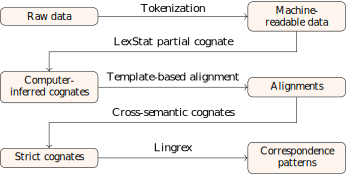
\includegraphics[width=0.8\textwidth]{calc-workflow.pdf}
  \caption{Current state-of-the-art workflow developed in collaboration of different research groups
  working in computer-assisted frameworks.}
  \label{fig:workflow}
\end{figure}

Although the workflow can be carried out almost completely without any manual intervention by a
linguist, we emphasize that this workflow explicitly \emph{allows} for expert intervention at
\emph{any} of the five stages. While, in our experience, specific care is required when lifting the
data the first time to machine-readable format, it should further be noted that \emph{all} steps of
the workflow profit from human intervention, since none of the automatic methods currently available
to us could spot all patterns in linguistic data without over- or underestimating their importance
for linguistic reconstruction.

Our workflow starts from \emph{raw data}, including tabular data from fieldwork notes or data
published in books and articles, which we re-organize and re-format in such a way that the data can
be processed by our tools. Once we have \emph{machine-readable data}, we can use methods for
automatic cognate detection \citep{List2016g} in order to infer \emph{partial cognates} across the
languages in our data. Having inferred cognates, we can now also align the data in the cognate sets.
While we could use phonetic alignment approaches discussed in the literature \citep{List2014d}, we
now use a new approach, based on phonotactic templates, which has the advantage of being much
faster and accurate when dealing with alignments for South-East-Asian languages. Once having
identified the alignments, we start to search automatically for cognates \emph{across} different
concepts. Since all automatic methods \emph{need} to start searching for cognates within the same
concept slot (otherwise, there would be too many false positives), our new method, which makes used
of a systematic comparison of readily aligned cognate sets, systematically searches for cognates
independent of their meaning. The improved, cross-semantic cognate sets, which are all readily
aligned, have the specific property of being \emph{strict}: no cognate set could compare two
morphemes from the same language which would differ in their pronunciation. \citep{List2018PBLOG7}
calls these cognate sets \emph{regular}, but in discussions with Nathan Hill, we decided that
\emph{regular} is probably not the best term, as they can well be wrong, so we call them
\emph{strict} now. Once strict cognates have been identified, we use the new algorithm for the
automatic inference of sound correspondence patterns across multiple languages by \citet{List2019a}
to infer the correspondence patterns in the data.

In Section \ref{sec:wf}, we will provide detailed examples how all steps of the workflow interact,
using a relatively recent collection of linguistic data on Hmong-Mien languages \citep{Chen2012} for
this purpose.
\subsection{Materials and Methods for the Workflow Illustration}

The data we use to illustrate our workflow in the next section was originally collected by
\citet{Chen2012}, and later added in digital form to the Wiktionary project. Chén's collection of
\emph{frequent terms} (\emph{chángyòng cíbiǎo 常用词表}, pp. 567-862) comprises 885 different
concepts translated into 25 varieties of Hmong-Mien. In Figure \ref{fig:data}, we contrast one
exemplary page from Chéns book with the data as it has been prepared by the Wiktionary users.
We can see that the data is essentially the same, but that the rows and columns of the tabular form
have been swapped.

\begin{figure}[htb]
  \centering
  \includegraphics[width=\textwidth]{chen-illustration.pdf}
  \caption{Contrasting Chén's original data with the table in Wiktionary}
  \label{fig:data}
\end{figure}

All methods have either been implemented and published before, or are shared along with the slides
and the handout for this talk. Since this is work in progress, however, we warn users that both data
and code will be in flux for some time, but we will make sure that both data and code can always be
readily analyzed with our tools. All code, the data we use, and installation instructions can be
found at \url{https://github.com/lingpy/calc-workflow}. We ask those interested in testing our
methods to use our issue-tracker on GitHub in case they face difficulties of any kind.
In this talk, we present the workflow with a subset of 10 varieties of the Hmong-Mien languages in
Chén's sample, for which we selected a subset of 313 concepts. The concepts were selected by
checking the overlap with the current 504 concept list of the Burmish Etymological Database project
(headed by Nathan W. Hill, data online at \url{https://dighl.github.io/burmish}). 
The languages were selected for some general reasons, like lexical coverage, geographic
distribution, or basic diversity, but not with the specific ``eye" of a historical linguist who
would select languages to explore the history of a language family. We would be glad about any additional
recommendations, if scholars feel competent to give us advice in this context.
The
geographic locations are shown in the Figure \ref{fig:geo}.

\begin{figure}[htb]
  \centering
  \includegraphics[width=\textwidth]{Geographic.pdf}
  \caption{Language geographic locations}
  \label{fig:geo}
\end{figure}

\section{Illustration of the Workflow}\label{sec:wf}
\subsection{From Raw Data to Segmented Data}
When comparing languages within a computer-assisted framework, with the goal of identifying sound
correspondence patterns in the data, we need to make sure that our data is machine-readable at
first. If the data is not machine-readable, we can neither use web-based tools like EDICTOR which
make it easy to edit the data \emph{manually} \citep{List2017d}, nor can we use computational tools,
like LingPy \citep{List2018i}, which can help us a great deal in identifying cognate sets and
aligning our data.

A first problem for many researchers is to get used to our formats for data representation. 
In contrast to the typical style used by scholars, we do not use simple tables, with languages in a
row and concepts in a column, or vice versa, but instead a so-called long-table format, in which we
reserve a \emph{row} in a table for each word, and add a er, which tells us what the cells in
each column contain in terms of the data. This long-table format reflects the rule of
``One Value per Cell'', as stated by the Cross-Linguistic Data Formats initiative
\citep{Forkel2018a}, reproduced in Figure \ref{fig:onevalue}. 

\begin{figure}[htb]
  \centering
  \includegraphics[width=0.75\textwidth]{one-value-per-cell.png}
  \caption{Long-table format instead of condensed formats with multiple values per cell.}
  \label{fig:onevalue}
\end{figure}

As a second rule, we have certain format specifications that make it easier form machines to deal
with our input. This includes

\begin{itemize}
  \item the use of a \emph{segmented} form of IPA transcriptions, in which a space is used to
    separate distinct sounds from each other, to give the computer direct information on whether
    symbol combinations are meant to reflect one sound (e.g., affricates, such as {\sil [ts, tʃ]}),
    or multiple sounds (compare German \emph{Handschuh} {\sil [h a n t ʃ uː]} vs. German
    \emph{Tschüss} {\sil [tʃ y s]}),
  \item them use of morpheme segmentation markers (we use a \texttt{+}) to indicate morpheme
    boundaries, which is straightforward when working with many morpheme-syllabic SEA languages, in
    which morphemes coincide with syllables,
  \item a clear-cut account on the concepts in our data, as they serve as the initial comparanda, so
    each concept needs to be given a clear-cut definition, and our preferable starting points are
    concept lists which are translated into the languages to be investigated, as opposed to
    pre-selected accounts on potential etymological items.

\end{itemize}

We indicate words in the computer-readable form, by adding a column called \texttt{TOKENS} in which
data is segmented with a space to distinguish different sounds, and with the plus-symbol to
distinguish different morphemes. 

Thus, our original data consists of a text-file, separated by tabstop, with the first row serving as
a header, and the following rows providing information for one word per language. Our software
requires the following columns to be submitted:

\begin{itemize}
  \item \texttt{ID}: numerical identifier, greater than 0,
  \item \texttt{DOCULECT}: name of the language,
  \item \texttt{CONCEPT}: some gloss for the concept,
  %\item VALUE: original form of the data,
  %\item FORM: the form in the data after correcting errors, or multiple forms-per-cell problems,
  \item \texttt{TOKENS}: the morpheme and sound-segmented form of the data.
\end{itemize}

We recommend also to add a column called \texttt{VALUE}, containing the original data, as well as a
column \texttt{FORM}, which shows the original data but corrected for multiple values per cell. The
software usually automatically creates a form \texttt{IPA}, which is not necessarily used, but a
legacy form that will be replaced by the \texttt{FORM} in future updates.
Additional values are then consistently added by our workflow and will be discussed later.
 
Note in general, the data can be prepared with typical spreadsheet programs, such as Excel or
LibreOffice or GoogleDocs. In order to create the textfiles, we recommend to simply copy-paste the
data from a spreadsheet by opening an empty text file, copying the data, and pasting it into the
file. In this way, the tab-separated format required by our applications will always be preserved.
 
We offer procedures to ease the conversion of the data to the required formats. While the creation
of long-table formats is usually done by applying a custom script, we use \emph{orthography
profiles} to create morpheme-segmented IPA representations for our \texttt{TOKENS} column from the
original data \citep{Moran2018}. Orthography profiles are a very straightforward way to convert raw
data to space-separated IPA representations. An orthography profile can be thought of as a simple text file with two or more columns in which the first
represents the values as you find them in your data (i.e., non-IPA transcriptions, etc.), and the other
columns allowing you to convert the sequence of characters that you find in the first column. So in brief,
you have a source-pattern and a replacement pattern, for example, the one shown in Table
\ref{tab:profile}. With such a replacement pattern, an input string \texttt{čashaa} would on the one
hand be segmented into \texttt{č a sh aa} and at the same time, it would be converted to \texttt{ tʃ
a ʃ aː}. We now offer an online demo of orthography profiles at
\url{http://calc.digling.org/profile}, which can be used to test and apply customized orthography
profiles.

\begin{table}[htb]
  \centering
  \tabular{ll}
  \textbf{Grapheme} & \textbf{IPA} \\
  č &  tʃ \\
  ž & dʒ\\
  th&  tʰ\\
  dh&  d̤\\
  sh&  ʃ\\
  a & a\\
  aa&  aː\\
\endtabular
\caption{Very simple orthography profile example.}
\label{tab:profile}
\end{table}

\begin{center}
  \tabular{|p{14cm}|}\hline
  SUMMARY \\\hline
  \begin{itemize}
    \item Data must be machine-readable in order to be amenable for computer-assisted analyses.
    \item Data must specifically be segmented, both with respect to the morpheme boundaries and the
      boundaries between distinct sounds.
    \item Data must be provided in form of a \emph{long table} with some specific column headers,
      providing all relevant information.
    \item Computer-assisted tools help to prepare the data for computer-assisted processing.
  \end{itemize}\\\hline
  \endtabular
\end{center}

\subsection{From Segmented Data to Cognate Sets}\label{sec:pcogs}

Once the data is segmented and provided in the long table format as it is required by the LingPy
software package, as described in our tutorial \citep{List2018f}, we can use LingPy's partial
cognate detection method to infer partial cognates in our linguistic data. Partial cognates are
hereby understood as cognate assessments \emph{per morpheme} in our data, as opposed to cognate
assessments \emph{per word}. 
While it has always been clear to scholars working in the field of South-East Asian linguistics that
cognacy should rather be assigned on the level of the morpheme than on the level of full words,
given that the high degree of compounding would easily complicate the identification of cognate
relations, automatic methods, and specifically phylogenetic reconstruction approaches usually still
assume a rather naive one-word-one-cognate relation \citep{List2016f}. 

In our framework, we explicitly address this problem by adopting a numerical annotation format in
which each morpheme instead of each word form is assigned to a specific cognate set
\citep{Hill2017a}. This framework is illustrated in Figure \ref{fig:pcogs}, where we contrast word
forms for ``yesterday" in five Burmish varieties, indicating their detailed ``cognate relations". 
In the first ``traditional" style of cognate coding, we would proceed in a \emph{strict} way, only
allowing those words which are completely cognate in all their morphemes to be judged as cognates.
In the second, \emph{loose} cognate annotation, we judge all words that are in a \emph{connected
component} in our shared morpheme network to be cognate, and in the last column, we show our
explicit coding of partial cognacy, in which each morpheme is assigned to one cognate set.

\begin{figure}[htb]
  \centering
  \tabular{cc}
  \includegraphics[width=0.45\textwidth]{pcogs-1.png} &
  \includegraphics[width=0.45\textwidth]{pcogs-2.png} \\\endtabular
  \caption{Partial cognacy in Burmish language varieties and different ways of coding (see Hill and
  List 2017 and further explanations in the main text).
  coding.}
  \label{fig:pcogs}
\end{figure}

The software package LingPy offers a straightforward algorithm to detect and annotate partial
cognates in datasets formatted as long tables. This algorithm by \citet{List2016g} uses techniques for automatic sequence
comparison to create a network of similar morphemes for each meaning slot in a given dataset. It
then filters those concepts in consecutive stages, with the goal of avoiding that two or more
morphemes in the same word for the same language are assigned to the same cluster. In the end, the
algorithm outputs the cognate judgments in the same format as indicated above in Figure
\ref{fig:pcogs}, namely, but assigning each morpheme to a given number, with the number representing
that cognate set.

Note that this algorithm works quite well, although it is, of course, not infallible. It reaches
between 88 and 90 percent on a test datasets consisting of Bai dialects, Chinese dialects, and
dialects of Tujia. With more challenging datasets, the scores will surely drop, but we can expect
that the automatic cognate detection is in any case \emph{helpful}, as is easier to correct cognates
than to assign them from scratch.

In addition to the cognate detection algorithm, the EDICTOR web-based tool for computer-assisted
language comparison \citep{List2017d}, freely available at \url{http://edictor.digling.org}, can be
used to quickly inspect and correct computer-generated cognate sets, by providing a very convenient
interface that allows users to quickly assign morphemes to cognate sets. The interface is
illustrated in Figure \ref{fig:edipart}.

\begin{figure}
  \centering
  \includegraphics[width=\textwidth]{partial-cognates.png}
  \caption{Partial cognate annotation within the EDICTOR tool for the word for ``chin" in 10
  selected Hmong-Mien varieties.}
  \label{fig:edipart}
\end{figure}

\begin{center}
  \tabular{|p{14cm}|}\hline
  SUMMARY \\\hline
  \begin{itemize}
    \item For a realistic annotation of cognate sets, the annotation of partial cognates, by which
      morphemes are assigned to cognate sets, is the only realistic choice.
    \item Partial cognates can be automatically identified with help of software, openly available
      as part of the LingPy software library (\url{lingpy.org}, \citealt{List2018i}) and the
      algorithm by \citet{List2016g}.
    \item Partial cognates can be annotated consistently with help of the EDICTOR tool
      \citep{List2017d}, online available at \url{http://edictor.digling.org}.
    \item Partial cognates in these frameworks are assigned to morphemes occurring in words with the
      same meaning, both for algorithmic and for practical reasons.
  \end{itemize}\\\hline
  \endtabular
\end{center}

\subsection{From Cognate Sets to Alignments}
Algorithms for phonetic alignments in historical linguistics have been proposed since the 1990s
\citep{Covington1996,Covington1998}. The basic of an alignment is to arrange sequences in such a way
in a matrix
that corresponding segments are placed in the same column \citep{List2018d}. For the transparent
annotation of sound correspondences, alignments are a \emph{sine qua non}, there is no way around
them, even if scholars at times think otherwise. Since sound correspondences can only be annotated
and detected when comparing sound sequences (words, morphemes) in full, we need alignments to
identify them, specifically when working with more than just two languages. 
 
During the beginning of the second millenium, the methods for phonetic alignments have drastically
improved. Starting with the work by \citet{Kondrak2000} on pairwise alignments, we have now stable
algorithms for multiple alignments that yield accuracy scores almost comparable to the
differences we would expect between human annotators \citep{List2014d}. With EDICTOR
\citep{List2017d}, we also have a
tool that facilitates to align words across a larger number of languages, and the LingPy software
package \citep{List2018i} offers a very stable implementation of the Sound-Class-Based phonetic
Alignment algorithm \citep{List2012c}, which can be considered the current state of the art, as far
as multiple phonetic alignments are concerned.
 
Unfortunately, phonetic alignment algorithms are not perfect, and correcting alignments manually is
tedious, specifically when working in computer-assisted workflows, where one runs a computational
analysis and then has experts correct the results. If one changes one cognate set assignment, one
has to re-do the whole alignment analysis, and if the algorithm constantly gets something wrong,
this means that the researcher will need to correct the alignment ever and ever again, even when
only small changes to the data are undertaken. 
 
For this reason, we started to develop a new method for multiple phonetic alignments, specifically
targeted to SEA languages with restricted syllable structure, which allows us to align words without
actually aligning them. This method, which we call \emph{template-based alignments}, starts from the
simple observation that many SEA languages don't differ much in their syllable structure, allowing
us to capture which sound occurs in which position, and which sound should be compared to which
other sound, by simply adding another column to our wordlist file, which contains a layer for the
phonotactic structure of each syllable. These \emph{templates} are stored in a column which we call
\texttt{STRUCTURE}, for convenience, and they are arbitrary in so far as we allow users to represent
their template by any symbol sequence, as long as they respect our two-fold segmentation for
segmentized IPA-strings, which uses space for the segmentation of sounds, and the plus sign to
segment morphemes. 
 
For reasons of simplicity, we started from the well-known structure of Sinitic languages, which --
following \citet{Wang1996} --
assumes syllable templates consisting of an \emph{initial} (\texttt{i}), a \emph{medial}
(\texttt{m}), a \emph{nucleus} (\texttt{n}), a \emph{coda} (\texttt{c}), and the \emph{tone}
(\texttt{t}). In this schema, Chinese \emph{tàiyáng} {\sil [tʰ~ai~⁵¹ +  j~a~ŋ~³⁵]} would be
represented as \texttt{i~n~t + i~n~c~t}. Assuming that the syllable template of the ancestral
language we want to investigate did not differ much from this, we can now use the templates to
align words automatically, by simply starting from our general template, to which we align all
words, and then deleting those columns for the syllable positions which do not occur in the words
under comparison. This is illustrate in Figure \ref{fig:template}, where four words for ``seven" in
four Hmong-Mien languages are successively aligned with each other.

\begin{figure}[htb]
  \centering
  \resizebox{\textwidth}{!}{%
  \tabular{ccccc}
  \tabular{llll}
  \bfseries Doculect & 
  \bfseries Concept & 
  \bfseries Tokens & 
  \bfseries Structure 
  \\\hline\hline
  East Baheng                 & seven  &\sil tɕ a ³¹ &\ttfamily i n t \\
  West Baheng                 & seven  &\sil tɕ a ŋ ⁴⁴ &\ttfamily i n c t \\
  Chuanqiandian               & seven  &\sil ɕ a ŋ ⁴⁴  &\ttfamily i n c t \\
  Chuanqiandian (CG) & seven  &\sil s ã ²²    &\ttfamily i n t \\
 \endtabular & → &
 \tabular{ccccc}
  \bfseries\ttfamily i &
  \bfseries\ttfamily m &
  \bfseries\ttfamily n &
  \bfseries\ttfamily c &
  \bfseries\ttfamily t \\\hline\hline
  \sil tɕ &\sil - &\sil a &\sil - &\sil ³¹ \\
  \sil tɕ &\sil - &\sil a &\sil ŋ &\sil ⁴⁴ \\
  \sil ɕ  &\sil - &\sil a &\sil ŋ &\sil ⁴⁴  \\
  \sil s  &\sil - &\sil ã &\sil - &\sil ²²   \\
  \endtabular & → & 
  \tabular{cccc} 
  \multicolumn{4}{c}{\bfseries Alignment} \\\hline\hline
  \sil tɕ & \sil a &\sil - &\sil ³¹ \\
  \sil tɕ & \sil a &\sil ŋ &\sil ⁴⁴ \\
  \sil ɕ  & \sil a &\sil ŋ &\sil ⁴⁴  \\
  \sil s  & \sil ã &\sil - &\sil ²²   \\
  \endtabular
\endtabular}
\caption{Basic procedure for template-based alignment.}
\label{fig:template}
\end{figure}

The problem of this procedure is that it requires more input by the user, since templates should
ideally be manually assigned and checked for each word in the data. However, by now, we offer
different automatic and semi-automatic approaches the further help to create syllable templates
automatically. As a first possibility, extended orthography profiles can be used. In these profiles,
the data is analyzed in much more detail, offering larger chunks in the first column, which can then
be converted to a template at the same time when converting unsegmented strings to segmented
strings. Since our procedure also offers to capture the beginning and the end of a sequence, this
allows for a rather straightforward handling that is usually sufficient for datasets of moderate
size. We illustrate this procedure in Table \ref{tab:ortho2}. An alternative possibility is to use
the SinoPy library, a Python package for quantitative tasks in Chinese historical linguistics
\citep{List2018g} to create templates from input strings automatically. 

%As many SEA languages seem to have similar syllable structures as Sinitic languages, this phonotactic template can help us aligning the segmentations as well. For this task, we need a clear guideline to align the segmentations. For LingPy to align segmentations according to the template we set up, an orthography profile comes in handy for this aspect, to indicate the alignment rules, we use i, m, n, c and t to represent Initial, Meidial, Nucleus, Coda (ending) and Tone in the profile. 

\begin{table}[htb]
  \centering
\begin{tabular}{llll}
\bfseries Grapheme & 
\bfseries Segmented & 
\bfseries IPA   & 
\bfseries Structure \\\hline\hline
\sil \^tʰ & \sil tʰ    & \sil tʰ    & \ttfamily i \\
\sil \^v  & \sil v     & \sil v     & \ttfamily i \\
\sil ɛ    & \sil ɛ     & \sil ɛ     & \ttfamily n \\
\sil au   & \sil au    & \sil au    & \ttfamily n\\
\sil iei  & \sil i ei  & \sil j ei  & \ttfamily m n \\
\sil oŋ   & \sil o ŋ   & \sil o ŋ   & \ttfamily n c \\
\sil uɑŋ  & \sil u ɑ ŋ & \sil w ɑ ŋ & \ttfamily m n c \\
\sil loŋ  & \sil l o ŋ & \sil l o ŋ & \ttfamily m n c \\
\sil ³¹\$ & \sil ³¹    & \sil ³¹    & \ttfamily t \\
\end{tabular}
\caption{An example of an orthography profile that can creates templates along with the conversion
to segmented IPA. The second column represents the data as we find it in the source, in segmented
form, the third column contains a certain amount of corrections for IPA handling, and the fourth
column offers the data in form of the phonotactic structure.}
\label{tab:ortho2}
\end{table}
 
Template-based alignments have not been extensively tested so far, although it is clear for our
purpose, that they work at a level of 100\%, given that the user virtually provides the alignment
without actually aligning sequences. We can think of additional experiments, in which our approach
to template-based alignments could be tested, also when dealing with languages with more complex
syllable structures, where longer, and more complex templates could be used along with our
algorithm. Since morphemes -- in contrast to words -- tend to be small, the major message
of our template-based alignment approach is that we do not need to invest too much time in
sophisticated algorithms that try to guess in whatever way how to arrange sound sequences in a
matrix, if we can -- at least for certain language families -- already determine how to align the
strings by simply looking at their phonotactics. Since template-based alignments are essentially
linear with respect to their computational complexity, template-based alignments may also provide
further help in all those tasks in computational historical linguistics, where alignments are
needed, but slow down the algorithms, as for example, when searching for regular sound
correspondences with help of randomizing the data \citep{List2012b}.

\begin{center}
  \tabular{|p{14cm}|}\hline
  SUMMARY \\\hline
  \begin{itemize}
    \item Alignments are indispensable for the detection of sound correspondence patterns.
    \item Given that existing algorithms are complex, not error-free, and difficult to apply, we use
      a new method, that essentially uses phonotactic templates, along with a meta-template to align
      morphemes in our data..
    \item The advantage of the method is that it is almost error-free (as long as the templates are
      correct), and extremely fast to apply.
    \item The disadvantage of the method is that it requires more user-input, since the templates
      need to be checked manually.
    \item In order to create templates from segmented data, two methods are available, (a)~extended
      orthography profiles, and (b)~a Python function provided along with the SinoPy Python library.
  \end{itemize}\\\hline
  \endtabular
\end{center}
\subsection{From Alignments to Cross-Semantic Cognates}
As mentioned above in Section \ref{sec:pcogs}, the partial cognates are only identified for words
with the same meaning. This is being done for algorithmic reasons (it would become quite complex to
compare all morphemes against each other algorithmically), and for practical reasons, since we
believe that it is always better to start from the obvious and save etymologies in historical
linguistics, rather than to start from complex ones. Given that semantic shift is a phenomenon for
which we dispose of little knowledge with respect to its patterns, we agree explicitly with scholars
like \citet{Dybo2008} in emphasizing that we should always expect to find clear-cut etymologies
within words of the same meaning, even if we know that more etymologies could be find when searching
\emph{cross-semantically}, i.e., among words which differ with respect to their meanings.
 
There are only a few approaches that try to identify cognates across different concepts, and one
could say that the task of \emph{cross-semantic cognate detection} is still one of the open problems
in computational historical linguistics. Approaches proposed so far include a rather complex
workflow by \citet{Wahle2016}, who uses \emph{hidden Markov models} for sequence comparison, and
proxies on colexifications, drawn from the database by \citet{Dellert2017}, to infer cognates across
different meaning slots. As this task is not completely evaluated, and only described in a short
paper, it is difficult to access its usefulness for our purposes. Another approach is presented by
\citet{Arnaud2017}, who apply Support Vector Machines trained on form and semantic similarities of
word pairs along with a flat clustering algorithm to partition words into cognate sets. 
While this approach is publicly available and seems to yield promising results, we are not sure to
which degree it would help us with our very specific goals of lifting an initially ``raw" dataset
to a level where we can assess sound correspondence patterns across multiple languages, especially
since the algorithms the authors use for cognate detection do \emph{not} take regular sound
correspondences into account, and they are also \emph{not} sensitive to partial cognates.
 
Thus, instead of these previously proposed solutions, we propose our own, rather simple approach to
search for cross-semantic partial cognate sets in our data. This approach is based on the
well-observed fact that the majority of morphemes in South-East Asian languages with a certain
preference for compounding and a high degree of word formation, is highly \emph{promiscuous}
\citep[8f]{List2016h}, given
that they recur within different words, surfacing in the form of \emph{partial colexifications}
\citep[62]{Hill2017a}. The term \emph{partial colexification} hereby serves as a cover term for
morphemes recurring across the lexicon of a language, with no specific distinction being made if
they are polysemous or homophonous. 
 
Our search for partial colexifications would not allow us directly to identify cross-semantic
cognates consistently, given that sound change may yield different morpheme mergers across different
languages. As a result, we cannot take the information from one language alone, but have to smartly
summarize all the information on recurring morphemes we can find in our data. The solution for this
problem is nevertheless straightforward, and it builds on the idea to not only compare single words, as originally proposed in \citet{Hill2017a}, but to compare complete \emph{alignments} instead. As our data is already aligned, and we have identified
cognates in a first run, potentially even refined by experts, we can compare whole cognate sets that
contain \emph{identical words in the same language}. 

If two alignments are completely identical with respect to the words they contain, 
there is no reason
to assign them to different cognate sets, and we can directly assign them to the same cognate class.
Even if they are simply homophonous, the assumption of regular sound change will allow us to treat
them similarly if we reconstruct the words back to the ancestral language.

The problematic cases are those cases, where we have \emph{incomplete data}. And this is usually
rather the rule than the exception.  We often will encounter cases where we have two alignments
which are only filled in parts with data from the different languages, and we will usually have
\emph{missing data} for one or more of the languages in our sample in a given alignment. Thus, when
comparing two alignments with each other, we need to make sure that we have at least one word in one
language in common. 

As an example, consider the data on ``son'' and ``daughter'' in five language varieties of our
illustration data. As can be seen immediately, two languages show striking \emph{partial
colexifications} for the two concepts, Chuanqiandian and East Qiandong. In both cases, one morpheme
recurs in the words for the two concepts. In the other cases, we find different words, but if we
compare the overall cognacy, we can also see that all five languages share one cognate morpheme for
``son'' (corresponding to the Proto-Hmong-Mien {\sil *tu̯ɛn} in Ratliff's reconstruction), 
and three varieties share one cognate morpheme for ``daughter'' (corresponding to {\sil
*mphje\textsuperscript{D}} in Ratliff's 2010 reconstruction), with the morpheme for ``son''
occurring also in the words for ``daughter'' in East Qiandong and Chuanqiandian, as mentioned
before.\nocite{Ratliff2010}


\begin{table}[htb]
  \centering
  \resizebox{\textwidth}{!}{%
  \tabular{lllll}\hline
  \bfseries Language &
  \bfseries Concept &
  \bfseries Form &
  \bfseries Cognacy &
  \bfseries Cross-Semantic \\\hline\hline
  East Baheng                     & SON      & \sil \colorbox{lightgray}{taŋ³⁵}         & 1     & 1 \\
  East Baheng                     & DAUGHTER & \sil pʰje⁵³                              & 2     & 2 \\\hline
  West Baheng                     & SON      & \sil ʔa³/⁰ + \colorbox{lightgray}{taŋ³⁵} & 3 1   & 3 1 \\
  West Baheng                     & DAUGHTER & \sil ta⁵⁵ + qa³/⁰ + tʰjei⁵³              & 4 5 6 & 4 5 6 \\\hline
  Chuanqiandian                   & SON      & \sil \colorbox{lightgray}{to⁴³}          & 1     & 1\\
  Chuanqiandian                   & DAUGHTER & \sil ⁿtsʰai³³                            & 7     & 7 \\\hline
  Chuanqiandian (Central Guizhou) & SON      & \sil tə²/⁰ + \colorbox{lightgray}{tə̃²⁴}  & 8 1   & 8 1\\
  Chuanqiandian (Central Guizhou) & DAUGHTER & \sil \colorbox{lightgray}{tə̃²⁴} + ⁿpʰe⁴² & 9 2   & 1 2\\\hline
  East Qiandong                   & SON      & \sil \colorbox{lightgray}{tei²⁴}         & 1     & 1 \\
  East Qiandong                   & DAUGHTER & \sil \colorbox{lightgray}{tei²⁴} + pʰa³⁵ & 9 2   & 1 2\\\hline
\endtabular}
  \caption{Terms for ``son'' and ``daughter'' across five Hmong-Mien varieties.}
  \label{tab:son}
\end{table}

Our workflow for automatically identifying these cases of cognacy is a new algorithm for
cross-semantic cognate detection, developed first for the work in the Burmish Etymological
Dictionary project lead by Nathan W. Hill. In this workflow, we start from all aligned cognate sets
in our data, and then systematically compare all alignments with each other. Whenever two
alignments are \emph{compatible}, i.e., they have (1)~at least one morpheme in one language
occurring in both aligned cognate sets, which is (2)~identical, and (3)~no shared morphemes in two
alignments which are \emph{not} identical, we treat them as belonging to one and the same cognate
set. We iterate over all alignments in the data algorithmically, merging the alignments into larger
sets in a greedy fashion, and re-assign cognate sets in the data. 

The results can be easily
inspected with help of the EDICTOR tool, for example, by inspecting cognate set distributions in
the data. When inspecting the cross-semantic cognates, which we label \texttt{CROSSIDS} in our data,
the tool will always show, which cognate sets span more than one concept, and users can directly
filter the data and look at the relevant instances. Among the 64 cognate sets reflected in all
languages in our sample, we find quite a few cross-semantically recurring morphemes, seven in total
(with many more for the whole data). The results are shown in Table \ref{tab:cross}.

\begin{table}[htb]
  \centering
  \tabular{llll}\hline
  Language &
  Concept &
  Form & 
  Morphemes \\\hline\hline
  East Baheng & NOSE & ⁿpjau³¹ & \texttt{NOSE} \\
  East Baheng & NASAL MUCUS & qa³/⁰ + ⁿpjau³¹ & \texttt{qa NOSE} \\\hline
  West Luobuohe & TWO & ʔu³¹ & \texttt{TWO} \\\hline
  West Luobuohe & TWENTY & ʔu³¹ + ʑo³¹ & \texttt{TWO zo} \\\hline
  West Baheng & SON & ʔa³/⁰ + taŋ³⁵ & \texttt{SON} \\
  West Baheng & SON-IN-LAW & taŋ³⁵ + wei³¹ & \texttt{SON wei} \\
  West Baheng & GRANDSON & taŋ³⁵ + seŋ³¹ & \texttt{SON seng} \\\hline
  East Qiandong & SUN &  qʰaŋ³³ + nei²⁴ & \texttt{po SUN} \\
  East Qiandong & DAY (NOT NIGHT) & nei²⁴ & \texttt{SUN} \\\hline
  West Baheng & FAECES (EXCREMENT) &  qa³¹ & \texttt{SHIT} \\
  West Baheng & STOMACH & ʔa³/⁰ + tɕʰi³⁵ + qa³¹ & \texttt{a tci SHIT} \\\hline
  West Qiandong & ANT & kæ̃⁴⁴ + mjɔ²² & \texttt{INSECT mjo} \\
  West Qiandong & EARTHWORM &  kæ̃⁴⁴+tɕuŋ⁴⁴ & \texttt{INSECT tsung} \\\hline
  East Baheng & BIRD & taŋ³⁵ + nuŋ³¹ & \texttt{BIRD-A BIRD-B} \\
  East Baheng & NEST & ʑo¹¹ + taŋ³⁵ + nuŋ³¹ & \texttt{zo BIRD-A BIRD-B} \\\hline
  \endtabular
  \caption{Partial cognates among stable concepts with reflexes in all languages in our test
  datasets. We highlight shared cognates by giving a tentative gloss for them in capital letters in
  the column \emph{Morphemes}.}
  \label{tab:cross}
\end{table}

\begin{center}
  \tabular{|p{14cm}|}\hline
  SUMMARY \\\hline
  \begin{itemize}
    \item For a realistic analysis, we need to identify cognates not only within the same meaning
      slot, but across different concepts, specifically when dealing with languages in which
      compounding and word formation are very productive.
    \item We employ a new method that makes use of a comparison of the alignments in readily
      identified and aligned partial cognate sets to identify those morphemes which recur across
      different concepts in our data.
    \item The results can be inspected with help of the EDICTOR, but not directly, by now, only
      indirectly with help of the browser for cognate sets.
    \item The interpretation of the results cannot be done automatically, but requires expert
      assessment with respect to the morphology of the data under consideration.
  \end{itemize}\\\hline
  \endtabular
\end{center}


\subsection{From cross-semantic cognates to correspondence patterns}
Having identified our cross-semantic cognates, or -- to be more specific -- our \emph{strict}
cross-semantic cognates, we can now finally run the analysis required to detect the sound
correspondence patterns in our data. Note that by sound correspondence \emph{patterns} we mean
essentially sound correspondences for more than just two languages. In most formal or automatic
approaches to historical linguistics, starting from \citet{Hoenigswald1960}, via
\citep{Kondrak2003}, up to the LexStat algorithm, which uses previously identified sound
correspondences to identify cognates across multiple languages \citep{List2012b}, sound
correspondences are exclusively handled for language \emph{pairs}, also when working with more than
two languages. This means, that instead of identifying correspondences across all languages in the
data, the methods or descriptions assume that it is enough to look at the correspondences for each
of the possible pairs in the data. While it is clear that computationally, this may be the only
feasible solution, especially when lacking further information or data about the languages, the
pairwise perspective does not help us to further proceed with respect to linguistic reconstruction.
If we wish to reconstruct the proto-language, we \emph{need} to switch to a multi-lingual
perspective, especially with respect to sound correspondences. For this reason, we adopt the term
\emph{correspondence pattern} for those cases where we have more than just two languages in our
data, and \emph{correspondence pattern detection} is the task by which we try to identify all
patterns of regular sound correspondences in our data. 
 
In our specific, alignment-based interpretation of sound correspondences, sound correspondence
patterns are understood as \emph{recurring alignment sites} in a given dataset.  An \emph{alignment
site} is a column in a given alignment, following the terminology that is usually employed by
biologists. While scholars occasionally share correspondence patterns in the literature, the way
they share them in almost never exhaustive, but always eclectic, being based on a pre-selection of
the data in such a way that they support a given theory or hypothesis.
 A prototypical example for
this representation is given in Figure \ref{fig:beekes}, with reflexes of Proto-Indo-European labial
and dental stops \citep[127]{Beekes1996}.
That does not essentially
mean that proposals on correspondence patterns in the literature are wrong per se, because scholars
often have good arguments to exclude specific patterns, which only occur due to specific sound
changes which are conditioned by peculiar contexts in some languages. It means, however, that
scholars do not always share all of the data, and as long as scholars do not share all of their
data, we do not have the possibility to assess whether they really know about all possible
variations that their data offers.

\begin{figure}[htb]
  \centering
  \includegraphics[width=\textwidth]{beekes1996.png}
  \caption{Example for the typical representation of correspondence patterns in the classical
  literature, taken from Beekes (1996: 127).}
  \label{fig:beekes}
\end{figure}

 
An example for a very transparent form of presenting a reconstruction along with correspondence
patterns is the Proto-Hmong-Mien reconstruction by \citet{Ratliff2010}. Ratliff herself talks about
\emph{correspondence sets}, listing a proto-sound following her reconstruction and all
\emph{reflexes} in the descendant languages, based on concrete cognate sets. An example for this
format, reflexes reflecting the initial {\sil *mbl-} in Proto-Hmong-Mien, is provided in Figure
\ref{fig:ratliff}. While this format is much more consistent than the one provided in Figure
\ref{fig:beekes} above, it still has a couple of disadvantages: (1)~it does not provide the full
words in the examples, but only the morphemes (something we track in our computer-assisted workflow,
by handling partial cognates consistently), (2)~it does not provide us with information on the
degree to which patterns are inconsistent, reflecting secondary variation in the individual
languages (we can only find that out by carefully inspecting the data ourselves), and (3)~the
representation is only to some degree machine-readable, not only because it is not digitized, but
also because we do not know completely to which correspondence pattern (or set) each of the other
sounds in the data belongs, and we will have problems to check the consistency of entire words when
given the data in this form.


\begin{figure}[htb]
  \centering
  \includegraphics[width=\textwidth]{ratliff2010.png}
  \caption{Example from Ratliff (2010: 57), correspondence pattern for Proto-Hmong-Mien {\sil *hn-}.}
  \label{fig:ratliff}
\end{figure}
 
The result of an correspondence pattern analysis as we imagine and propose it can be thought of as
some kind of a table, in which languages are placed in the columns, and correspondence patterns are
placed in rows, with each cell indicating for each individual correspondence pattern, which reflex
sound a given language shows for this pattern. If we further assume that our interface is
\emph{interactive}, the correspondence pattern analysis should further deliver all information in a
way that can be directly traced back to the original data, from the original morphemes, the position
in the syllable, up to the potential irregularity of the pattern, and its overall frequency in the
data under investigation. This format is essentially offered by the EDICTOR tool by now, when using
the correspondence pattern inspection panel of the tool, as illustrated in Figure \ref{fig:ede}.
Here, the user finds the correspondence patterns in the data sorted according to the number of
cognate sets in which they are reflected, along with an index indicating where in the alignment the
pattern occurs, with which other patterns it is compatible, and the concepts in which the
correspondence pattern is reflected. While this would not offer much advantages over any display in
books, the tool is interactive, and clicking on the patterns allows to see the full word, the
underlying alignment, or to quickly browse back to the original data. All in all, we can lift our
data easily to a level similar to the one provided in Ratliff's reconstruction, but without loosing
track of all steps that were done before.

\begin{figure}
  \centering
  \includegraphics[width=\textwidth]{edictor-hn.png}
  \caption{Interactive display of correspondence patterns within the EDICTOR tool.}
  \label{fig:ede}
\end{figure}
 
Correspondence patterns can be computed in two ways, either by using the correspondence pattern
detection algorithm by \citet{List2019a}, implemented in the LingRex package \citep{List2018j},
which will probably later be included as part of LingPy. An alternative is to use the EDICTOR
directly, although this algorithm is based on a simple sorting of alignment sites, and will have
difficulties when being confronted with particularly patchy data, with many missing reflexes for a
given cognate set.
 
When applying the algorithm by \citet{List2019a} to our data of 10 languages, we find as many as 786
patterns in total for all five different phonotactic positions that we were assuming for this
analysis. This may seem to be a lot, but it should be kept in mind that -- apart from errors in our
identification of cognate sets and alignments -- it is quite common to find a lot of exceptional
correspondence patterns, and even in Ratliff's data, we can see that essentially all four patterns
offered for Proto-Hmong-Mien {\sil *hn-} are different from each other in at least one reflex. 
We still expect that a certain amount, especially of the 323 patterns in our analysis which occur only once in the data, may result from the fact that we did only use computational analyses for the data analysis, without any human interaction. In general, however, we are confident, that our approach
could identify a quite substantial part of the patterns in the data, which is also confirmed by the comparison with Ratliff's work, which we qualitatively compared against our findings. 

\begin{table}[htb]
  \centering
  \tabular{llllllllllllll}
  \bfseries No. &
  \bfseries Concept &
  \bfseries Proto-Form &
  \bfseries 1&
  \bfseries 2&
  \bfseries 3&
  \bfseries 4&
  \bfseries 5&
  \bfseries 6&
  \bfseries 7&
  \bfseries 8&
  \bfseries 9&
  \bfseries 10&
  \bfseries 11\\\hline\hline
  \multicolumn{3}{c}{Pattern}                             &
  \sil n̥h & 
  \sil n̥h& 
  \sil hn̥ & 
  \sil n & 
  \sil n̥ & 
  \sil n̥ &  
  \sil n̥ & 
  \sil ? & 
  \sil n &
  \sil n̥ & 
  \sil n \\\hline\hline
  1 & grain head/bag    &\sil *hnɔn    &\sil n̥h   &\sil n̥h &\sil hn̥ & n & n̥ &\sil n̥    & n̥ &\sil Ø    &\sil n &\sil \cellcolor{lightgray} n &\sil  Ø\\
  2 & to hear           &\sil *hnəumX  &\sil n̥h   &\sil n̥h &\sil hn̥ & n & Ø &\sil n̥    & n̥ &\cellcolor{lightgray}\sil n &\sil n &\sil n̥    &\sil  Ø\\
  3 & to put on clothes &\sil *(h)naŋX &\cellcolor{lightgray}\sil n &\sil n̥h &\sil hn̥ & n & n̥ &\cellcolor{lightgray}\sil n &\cellcolor{lightgray}\sil n &\sil Ø    &\sil Ø &\sil Ø    &\sil  n\\
  4 & to cough          &\sil *hn ɔp   &\cellcolor{lightgray}\sil ŋ &\sil Ø  &\sil hn̥ & n & n̥ &\sil Ø    & Ø &\cellcolor{lightgray}\sil n̥ &\sil Ø &\sil n̥    &\sil  Ø\\
\endtabular
\caption{Irregularities in the patterns for Proto-Hmong-Mien {\sil *hn-} in the reconstruction of Ratliff (2010).}
\label{tab:regs}
\end{table}

As an example why we are confident that our workflows yield in fact very useful results, even when
applied in a purely automatic fashion, consider the pattern \#189 in our current account of the
data, as displayed in Figure \ref{fig:fruit}. The reflexes in this pattern correspond to Ratliff's Proto-Hmong-Mien {\sil *pr-} initial, and
our workflow allowed us to find four examples, including words for ``five'' and ``house'', which are
also the primary witnesses in Ratliff's reconstruction. Our algorithm for cognate detection
essentially succeeded in identifying that the words under question are cognate, despite their highly
divergent reflexes, including {\sil p-}, {\sil tʂ-}, {\sil ts-}, and {\sil t-}. The algorithm failed
to identify East Qiandong (\texttt{qia}) {\sil ts a ²⁴} as cognate with the other words for
``five'', but this can be easily corrected, specifically when inspecting the correspondence pattern,
as we would beyond doubt assume that the East Qiandong initial is {\sil ts-}. The final two forms, 
``fruit'' and ``bear fruit'' probably reflect cognate forms, but they could not be captured by our
cross-semantic cognate detection algorithm, since the words differ in tone, and can therefore not be
considered as being \emph{strictly} cognate. Ratliff assigns the words to another correspondence
pattern {\sil *pj-}, which is justified when assuming that this would yield traces in the reflexes
of our data. Indeed, when inspecting the data further, we can see that the algorithm missed
to assign Chuanqiandian {\sil ts i ⁵⁵} ``fruit'' to the other cognate sets, but if the algorithm had
done so, the ``fruit'' correspondence pattern would no longer be compatible with the ``five''
correspondence pattern and therefore no longer be listed here. 

\begin{figure}[htb]
  \centering
  \includegraphics[width=\textwidth]{five.png}
  \caption{Correspondence patterns for ``five'', ``house'', and ``fruit'', as automatically
  identified from our data for testing.}
  \label{fig:fruit}
\end{figure}

\begin{center}
  \tabular{|p{14cm}|}\hline
  SUMMARY \\\hline
  \begin{itemize}
    \item Correspondence patterns are similar to sound correspondences, but they are explicitly
      thought to be identified across multiple languages, by clustering the alignment sites in a
      given dataset.
    \item Correspondence patterns are indispensable for linguistic reconstruction.
    \item Apart from a tedious and not fully traceable manual identification of sound correspondence
      patterns, two computer-assisted methods for their identification from alignments are
      available: a (rather poor) built-in application provided by the EDICTOR tool, and a
      sophisticated variant, based on a network-algorithm by List (2019), provided as a Python
      package.
    \item The EDICTOR offers for a convenient inspection of inferred correspondence patterns, and
      allows scholars to directly see the consequences of their data analysis.
  \end{itemize}\\\hline
  \endtabular
\end{center}



\section{Discussion}

Our workflows are not complete yet, and they are also not perfect. Many more aspects need to be
integrated, discussed, and formalized. In the following, we will point to two important aspects,
namely, (a)~possible improvements of the algorithm, and (b)~general challenges for all future
endeavor in computer-assisted or computational historical linguistics.
\subsection{Possible improvements}
The possible improvements include to further integrate our preliminary attempts for
\emph{semi-automatic reconstruction}, starting from readily identified sound correspondence
patterns. Experiments are ongoing in this regard, but we have not yet had time to integrate it fully
so far. In general, our workflow also needs a clearer integration of automatic and manual
approaches, ideally accompanied by extensive tutorials that would allow users to start with the
tools without specifically getting in touch with us and asking us (although we tend to respond
quickly to all kinds of inquiries). We should also work on a better handling of output formats, both
for correspondence patterns, where we may want to produce some format similar to Ratliff's
representation, also to allow readers to make use of the format most convenient to them, and for
other aspects of the data. We should also further work on initial attempts on testing the
consistency of the data, be it with help of \emph{prediction experiments} \citep{Bodt2019PREPRINTa},
or with more elaborated quasi-probabilistic accounts that test how well a given word fits into a
given cognate set.

\subsection{General challenges}

General challenges include the full-fledged lexical reconstruction of words, i.e., a reconstruction
that would potentially also provide compounds in etymological dictionaries. While current
reconstructions (also Ratliff 2010) often only provide morphemes (and thus only carry out a
morpheme-based phonological reconstruction, instead of complete reconstructions of the words that
were potentially used in the languages before. Furthermore, we will need a convincing annotation of
sound change that would ideally allow us to even check which sounds changed when during language
history on which branch of the language.


\section{Outlook}

This draft has provided a rather detailed account on what we consider the current state-of-the-art
in computer-assisted language comparison. Starting from raw data, we have shown how these can be
successively lifted to higher levels of annotation. While our five-step workflow can be safely
applied purely manually, purely automatically, or in a computer-assisted manner, we have shown that
even with a pure automatic approach, one can already get quite far in \emph{computer-assisted
language comparison.} In the future, we hope to further enhance the workflows and make them more
accessible to users from different backgrounds.

\nocite{List2019a}

\printbibliography
\end{document}
